%%%%%%%%%%%%%%%%%%%%%%%%%%%%%%%%%%%%%%%%%%%%%%%%%%%%%%%%%%%%%%%%%%%%%%%%%%%%%%%%%%%%%%%%%%%%%%%%%%%%

\documentclass{article}

%%%%%%%%%%%%%%%%%%%%%%%%%%%%%%%%%%%%%%%%%%%%%%%%%%%%%%%%%%%%%%%%%%%%%%%%%%%%%%%%%%%%%%%%%%%%%%%%%%%%

\usepackage{tikz}
\usetikzlibrary{calc,positioning,shapes,shadows,arrows,decorations,decorations.pathmorphing,external}
\tikzexternalize % activate! & run "pdflatex -shell-escape test.tex"
\usepackage{pgffor}

%%%%%%%%%%%%%%%%%%%%%%%%%%%%%%%%%%%%%%%%%%%%%%%%%%%%%%%%%%%%%%%%%%%%%%%%%%%%%%%%%%%%%%%%%%%%%%%%%%%%

\begin{document}
%%%%%%%%%%%%%%%%%%%%%%%%%%%%%%%%%%%%%%%%%%%%%%%%%%%%%%%%%%%%%%%%%%%%%%%%%%%%%%%%
\tikzsetnextfilename{figure-scanner}
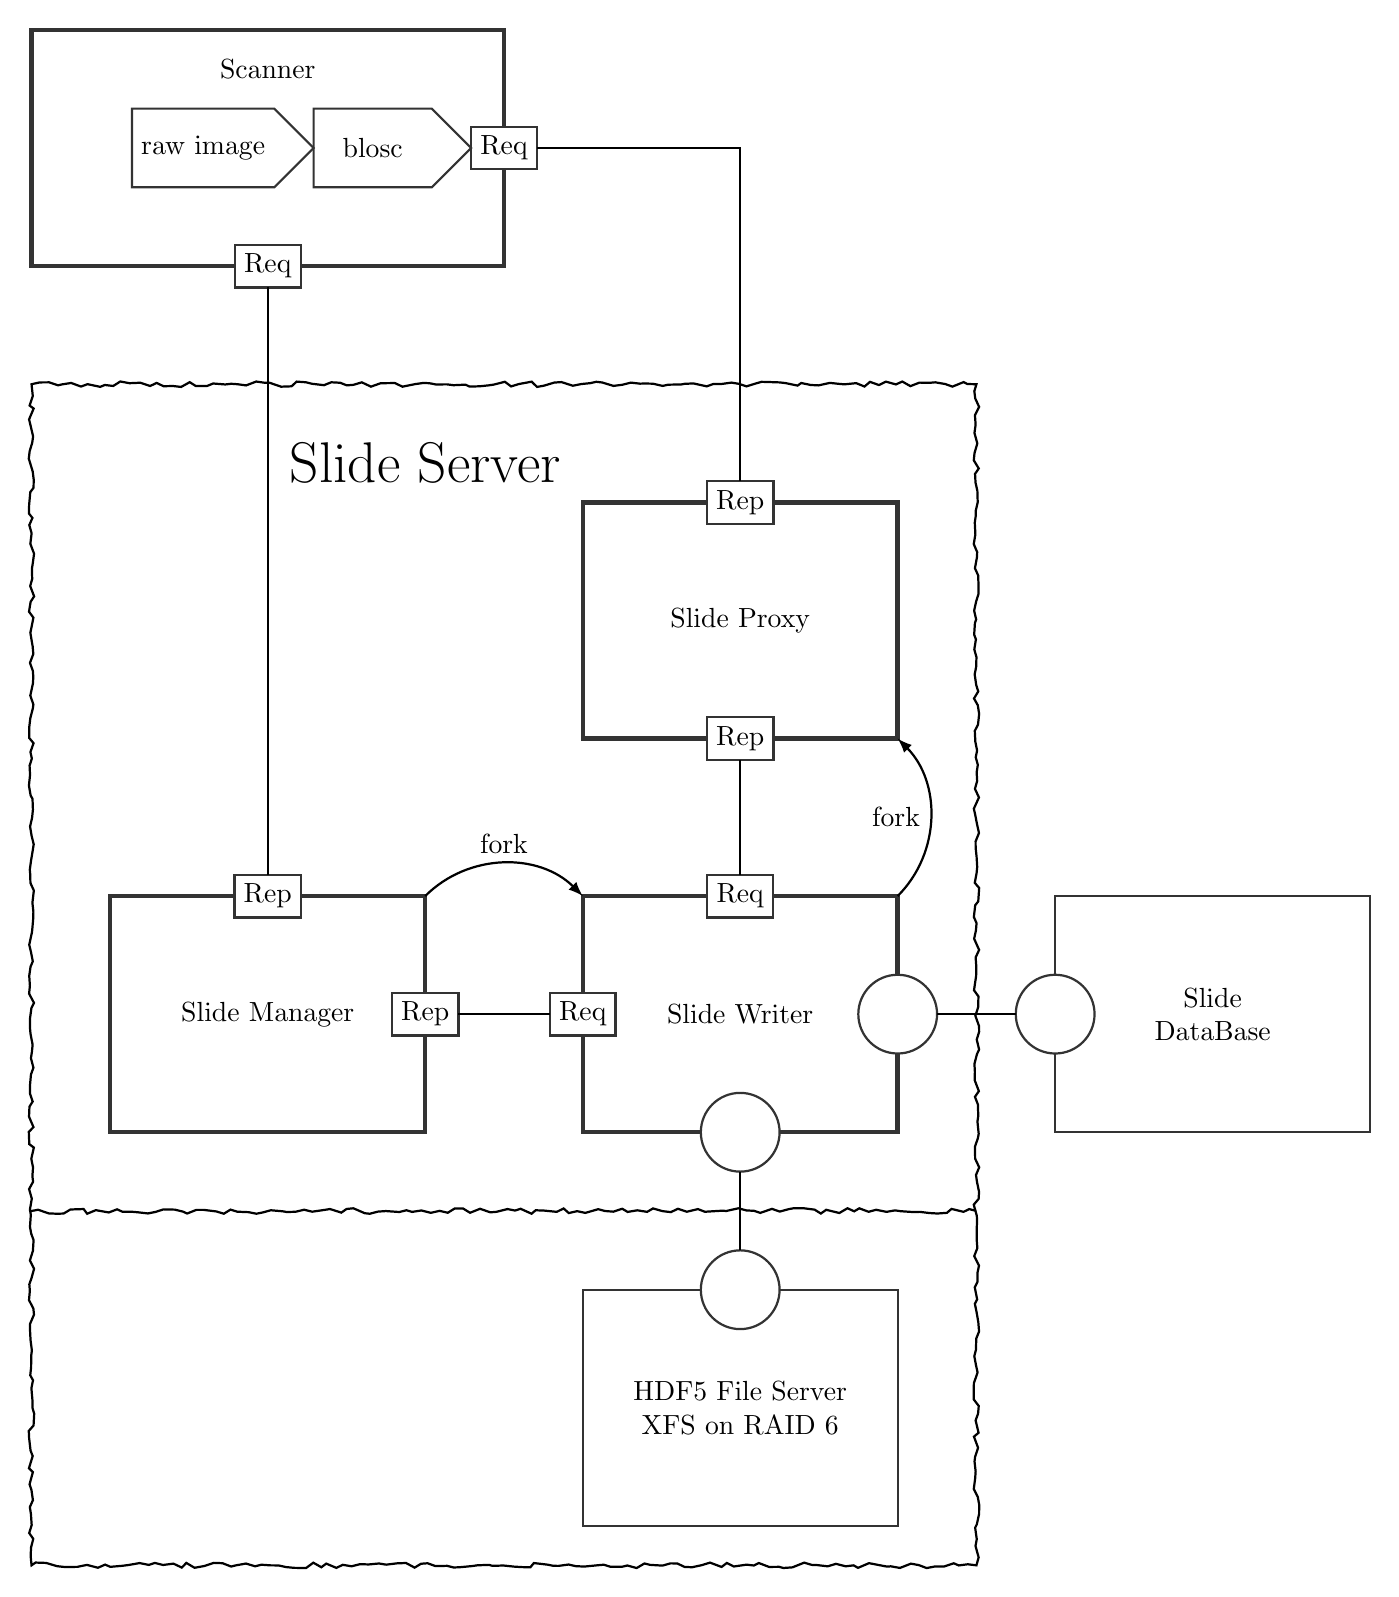
\begin{tikzpicture}[
  node distance=1cm, on grid,
  thick,
  scanner/.style={
    rectangle,
    fill=white!100,
    ultra thick,
    draw=black!80,
    minimum height=30mm, minimum width=60mm,
    outer sep=0pt
  },
  slide manager/.style={
    rectangle,
    fill=white!100,
    ultra thick,
    draw=black!80,
    minimum height=30mm, minimum width=40mm,
    outer sep=0pt
  },
  slide writer/.style={
    rectangle,
    fill=white!100,
    ultra thick,
    draw=black!80,
    minimum height=30mm, minimum width=40mm,
    outer sep=0pt
  },
  slide proxy/.style={
    rectangle,
    fill=white!100,
    ultra thick,
    draw=black!80,
    minimum height=30mm, minimum width=40mm,
    outer sep=0pt
  },
  file server/.style={
    rectangle,
    fill=white!100,
    thick,
    draw=black!80,
    minimum height=30mm, minimum width=40mm,
    outer sep=0pt,
    align=center
  },
  database/.style={
    rectangle,
    fill=white!100,
    thick,
    draw=black!80,
    minimum height=30mm, minimum width=40mm,
    outer sep=0pt,
    align=center
  },
  stage/.style={
    signal=to east,
    fill=white!100,
    thick,
    draw=black!80,
    minimum height=10mm, minimum width=20mm,
    outer sep=0pt
  },
  zmq socket/.style={
    rectangle,
    fill=white!100,
    thick,
    draw=black!80,
    minimum height=5mm, minimum width=5mm,
    outer sep=0pt
  },
  socket/.style={
    circle,
    fill=white!100,
    thick,
    draw=black!80,
    minimum height=10mm, minimum width=10mm,
    outer sep=0pt
  }
  ]
%\draw[help lines] (-5,-10) grid (15,15);
% Slide Manager
\node [slide manager] (slide manager) at (0,0) {Slide Manager};
\node [zmq socket] (scanner slide manager rep) at (slide manager.north) {Rep};
\node [zmq socket] (slide writer manager rep) at (slide manager.east) {Rep};
% Scanner
\node [scanner] (scanner) at (0,11) {};
\node at ($(scanner) + (0,1)$) {Scanner};
\node [zmq socket] (scanner proxy req) at (scanner.east) {Req};
\node [zmq socket] (scanner slide manager req) at (scanner.south) {Req} edge (scanner slide manager rep);
%\node [stage] (blosc) at ($(scanner proxy req.west) - (1.25,0)$) {blosc}; % [left=of scanner proxy req,xshift=-20mm]
%\node [stage] (blosc) [left=of scanner proxy req] {blosc};
%\node [stage] (raw image) at ($(blosc.west) - (1.5,0)$) {raw image};
\draw (scanner proxy req.west) node[stage,anchor=east] (blosc) {blosc};
\draw (blosc.west) node[stage,anchor=east] (raw image) {raw image};
% Slide Writer
\node [slide writer] (slide writer) at (6,0) {Slide Writer};
\node [zmq socket] (slide writer proxy req) at (slide writer.north) {Req};
\node [zmq socket] (slide writer manager req) at (slide writer.west) {Req} edge (slide writer manager rep);
\path[->,>=latex] (slide manager.north east) edge[bend left=45] node[above] {fork} (slide writer.north west);
\node [socket] (slide writer database) at (slide writer.east) {};
\node [socket] (slide writer file server) at (slide writer.south) {};
% Slide Proxy
\node [slide proxy] (slide proxy) at ($(slide writer.north) + (0,3.5)$) {Slide Proxy};
\node [zmq socket] (scanner proxy rep) at (slide proxy.north) {Rep};
\draw (scanner proxy rep) |- (scanner proxy req);
\node [zmq socket] (slide writer proxy rep) at (slide proxy.south) {Rep} edge (slide writer proxy req);
\path[->,>=latex] (slide writer.north east) edge[bend right=45] node[left] {fork} (slide proxy.south east);
% Database
\node [database] (database) at ($(slide writer.east) + (4,0)$) {Slide\\ DataBase};
\node [socket] (database socket) at (database.west) {} edge (slide writer database);
% File Server
\node [file server] (file server) at ($(slide writer.south) - (0,3.5)$) {HDF5 File Server\\XFS on RAID 6};
\node [socket] (file server socket) at (file server.north) {} edge (slide writer file server);
% Slide Server Host
\draw[decorate, decoration={random steps,segment length=3pt,amplitude=1pt}]
(-3,-7) rectangle (9,8)
(-3,-2.5) -- (9,-2.5);
\node at (2,7) {\huge Slide Server};
\end{tikzpicture}
%%%%%%%%%%%%%%%%%%%%%%%%%%%%%%%%%%%%%%%%%%%%%%%%%%%%%%%%%%%%%%%%%%%%%%%%%%%%%%%%
\tikzsetnextfilename{figure-viewer}
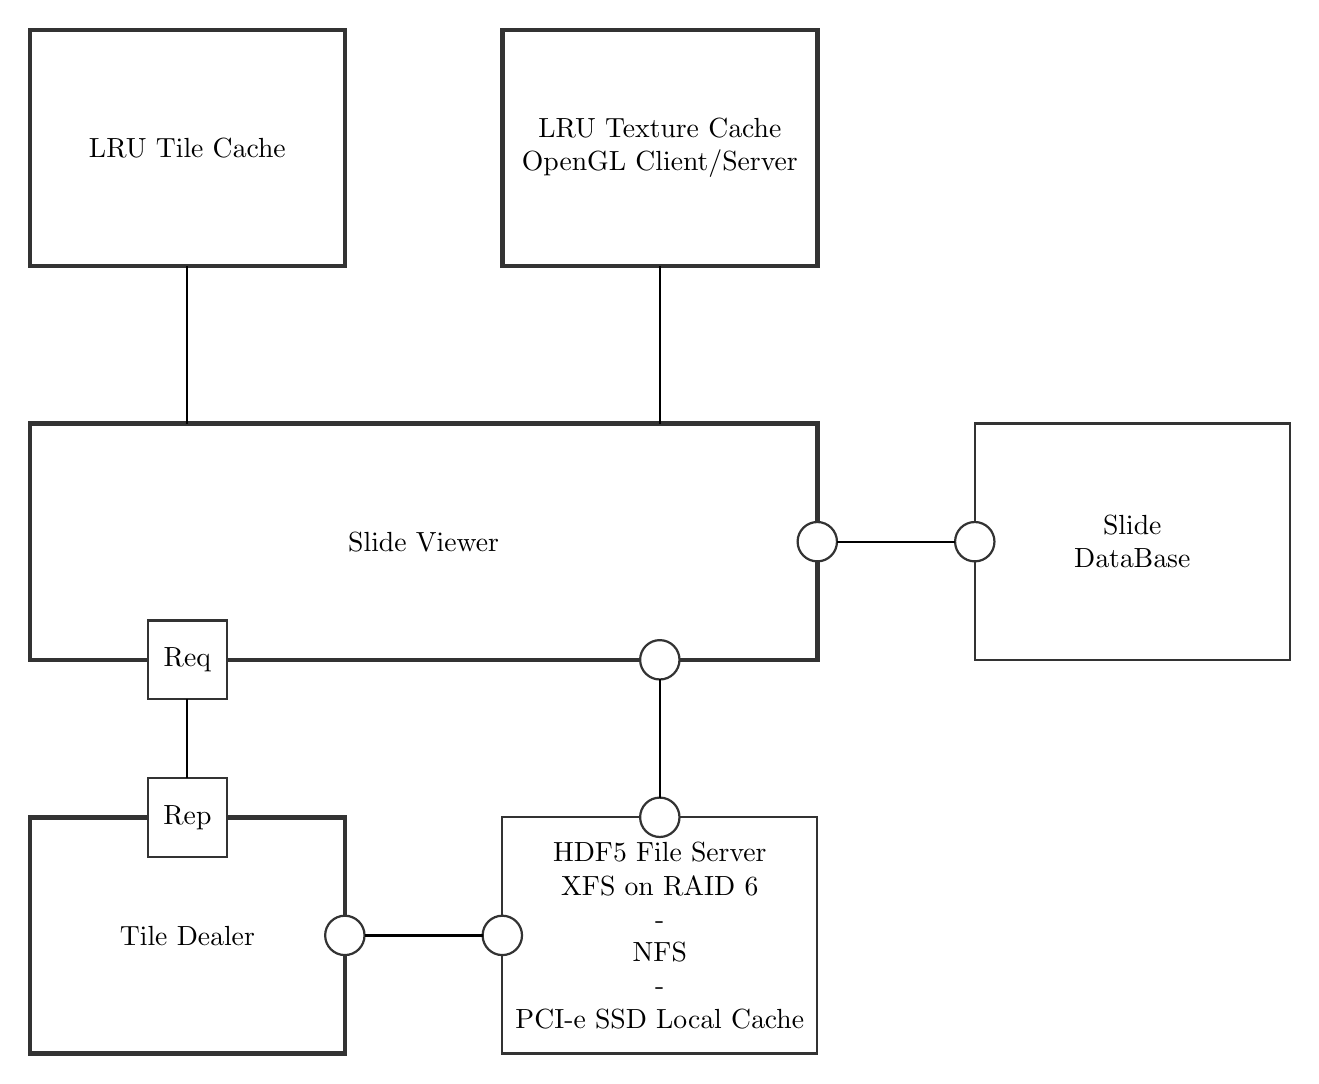
\begin{tikzpicture}[
  node distance=1cm, on grid,
  thick,
  slide viewer/.style={
    rectangle,
    fill=white!100,
    ultra thick,
    draw=black!80,
    minimum height=30mm, minimum width=100mm,
    outer sep=0pt
  },
  tile cache/.style={
    rectangle,
    fill=white!100,
    ultra thick,
    draw=black!80,
    minimum height=30mm, minimum width=40mm,
    outer sep=0pt
  },
  texture cache/.style={
    rectangle,
    fill=white!100,
    ultra thick,
    draw=black!80,
    minimum height=30mm, minimum width=40mm,
    outer sep=0pt,
    align=center
  },
  slide dealer/.style={
    rectangle,
    fill=white!100,
    ultra thick,
    draw=black!80,
    minimum height=30mm, minimum width=40mm,
    outer sep=0pt
  },
  file server/.style={
    rectangle,
    fill=white!100,
    thick,
    draw=black!80,
    minimum height=30mm, minimum width=40mm,
    outer sep=0pt,
    align=center
  },
  database/.style={
    rectangle,
    fill=white!100,
    thick,
    draw=black!80,
    minimum height=30mm, minimum width=40mm,
    outer sep=0pt,
    align=center
  },
  zmq socket/.style={
    rectangle,
    fill=white!100,
    thick,
    draw=black!80,
    minimum height=10mm, minimum width=10mm,
    outer sep=0pt
  },
  socket/.style={
    circle,
    fill=white!100,
    thick,
    draw=black!80,
    minimum height=5mm, minimum width=5mm,
    outer sep=0pt
  }
  ]
%\draw[help lines] (-5,-10) grid (15,15);
% Slide Viewer
\node [slide viewer] (slide viewer) at (0,0) {Slide Viewer};
\node [socket] (slide viewer database) at (slide viewer.east) {};
\node [socket] (slide viewer file server) at ($(slide viewer.south) + (3,0)$) {};
\node [zmq socket] (slide viewer dealer req) at ($(slide viewer.south) + (-3,0)$) {Req};
\coordinate (slide viewer tile cache) at ($(slide viewer.north) + (-3,0)$);
\coordinate (slide viewer texture cache) at ($(slide viewer.north) + (3,0)$);
% Tile Cache
\node [tile cache] (tile cache) at ($(slide viewer tile cache) + (0,3.5)$) {LRU Tile Cache};
\coordinate (tile cache socket) at (tile cache.south);
\draw (tile cache socket) -- (slide viewer tile cache);
% Texture Cache
\node [texture cache] (texture cache) at ($(slide viewer texture cache) + (0,3.5)$) {LRU Texture Cache\\ OpenGL Client/Server};
\coordinate (texture cache socket) at (texture cache.south);
\draw (texture cache socket) -- (slide viewer texture cache);
% Database
\node [database] (database) at ($(slide viewer.east) + (4,0)$) {Slide\\ DataBase};
\node [socket] (database socket) at (database.west) {} edge (slide viewer database);
% File Server
\node [file server] (file server) at ($(slide viewer file server) + (0,-3.5)$)
  {HDF5 File Server\\ XFS on RAID 6\\ -\\ NFS\\ -\\ PCI-e SSD Local Cache};
\node [socket] (file server socket) at (file server.north) {} edge (slide viewer file server);
\node [socket] (file server socket 2) at (file server.west) {};
% Slide Dealer
\node [slide dealer] (slide dealer) at ($(slide viewer dealer req) + (0,-3.5)$) {Tile Dealer};
\node [zmq socket] (slide viewer dealer rep) at (slide dealer.north) {Rep} edge (slide viewer dealer req);
\node [socket] (slide dealer file server) at (slide dealer.east) {} edge (file server socket 2);
\end{tikzpicture}
\end{document}

%%%%%%%%%%%%%%%%%%%%%%%%%%%%%%%%%%%%%%%%%%%%%%%%%%%%%%%%%%%%%%%%%%%%%%%%%%%%%%%%%%%%%%%%%%%%%%%%%%%%
%%% Local Variables: 
%%% mode: latex
%%% TeX-master: t
%%% End: 
%%%%%%%%%%%%%%%%%%%%%%%%%%%%%%%%%%%%%%%%%%%%%%%%%%%%%%%%%%%%%%%%%%%%%%%%%%%%%%%%%%%%%%%%%%%%%%%%%%%%
